\documentclass[11pt]{article}
\usepackage{amsmath, amssymb, graphicx, hyperref, caption}
\usepackage[margin=1in]{geometry}
\usepackage{float}
\setlength{\parindent}{0em}
\setlength{\parskip}{0.5em}

\title{CTA200 2025 Assignment 3}
\author{Mayesha Rahaman}
\date{May 13, 2025}

\begin{document}

\maketitle

\section*{Question 1}

To explore the Mandelbrot set, we iterated the relation $z_{i+1} = z_i^2 + c$ for each complex number $c = x + iy$ in the region $-2 < x < 2$, $-2 < y < 2$, starting from $z_0 = 0$. In the code, divergence was detected using the condition \texttt{np.abs(z) > 2}, which corresponds to $|z|^2 > 4$. This threshold guarantees divergence: once $|z| > 2$, the sequence will escape to infinity.

The function \texttt{iter\_func} implemented this iteration. It creates a 2D grid of complex numbers, iteratively updates $z \leftarrow z^2 + c$, and records the number of iterations until each point diverges (or reaches the maximum allowed). The function returns a 2D array that encodes the iteration step at which each $c$ diverged.

Two visualizations were produced: a binary map showing which points remained bounded vs. diverged, and a colored map where the color represents how quickly each point diverged. These plots reveal the intricate boundary of the Mandelbrot set and its fractal nature.

The results highlight the sensitivity near the boundary, where small changes in $c$ produce very different long-term behaviors. The divergence-time plot especially emphasizes the self-similarity of the set and reveals finer structural detail at the edges.

\begin{figure}[H]
    \centering
    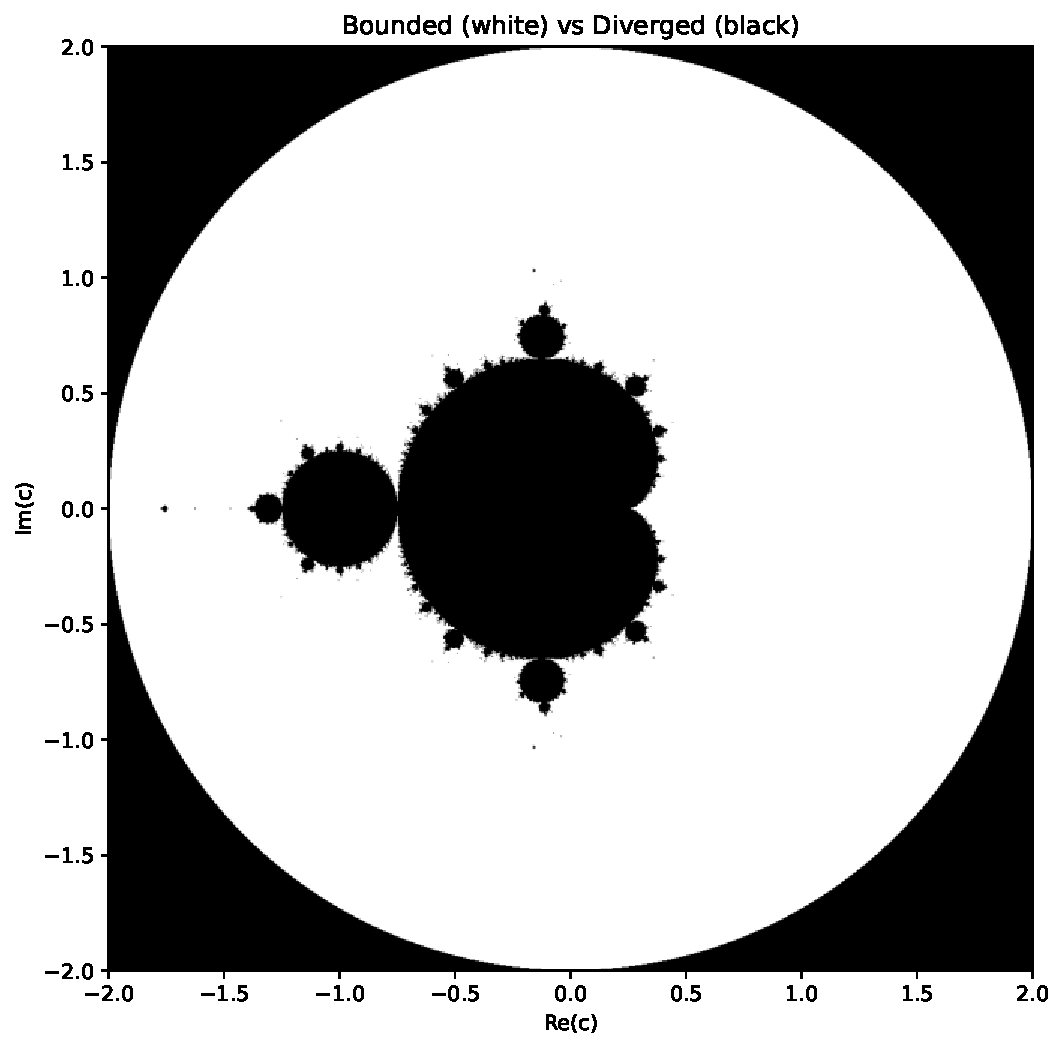
\includegraphics[width=0.45\textwidth]{fig1a.pdf}
    \hfill
    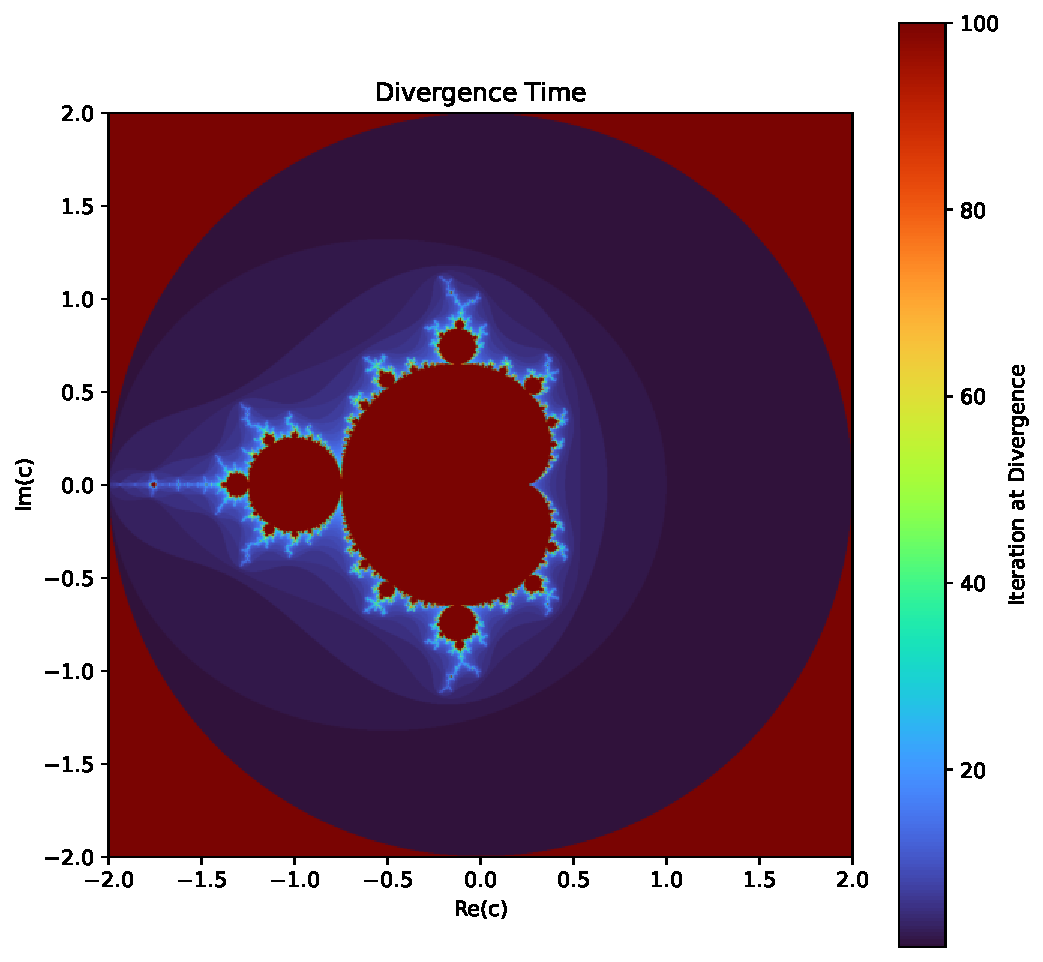
\includegraphics[width=0.45\textwidth]{fig1b.pdf}
    \caption{Left: Binary map showing bounded (white) vs. diverged (black) points in the Mandelbrot set. 
    Right: Escape-time plot, where color indicates the iteration at which divergence occurred.}
\end{figure}

\section*{Question 2.1}

We investigated the Lorenz system of differential equations, which model convection in the Earth's atmosphere under simplified conditions. The system is defined by three coupled nonlinear equations:
\[
\begin{aligned}
\dot{X} &= -\sigma (X - Y) \\
\dot{Y} &= rX - Y - XZ \\
\dot{Z} &= -bZ + XY
\end{aligned}
\]

The equations were implemented in Python as a function \texttt{lorenz(t, W, sigma, r, b)}. This function computes the time derivatives of the state vector $W = (X, Y, Z)$ and was passed to SciPy's \texttt{solve\_ivp} integrator. 

\section*{Question 2.2}

We used the standard values from Lorenz’s original 1963 paper: $\sigma = 10$, $r = 28$, and $b = 8/3$. We solved the system over the time interval $t = 0$ to $60$ using the initial condition $W_0 = [0., 1., 0.]$ and enabled dense output to support interpolation for later subparts.

This setup allowed us to reproduce Lorenz's original figures and analyze the system's sensitivity to initial conditions in the later parts of the question.

\section*{Question 2.3}

To recreate Lorenz’s Figure 1, we plotted the $Y(t)$ component of the system over the interval $t = 0$ to $30$, corresponding to the first 3000 iterations with a time step of $\Delta t = 0.01$. The plot was divided into three panels, each displaying a 10-second (1000-iteration) window to match the style of the original figure.

We used \texttt{matplotlib.pyplot.subplots} to generate three vertically stacked plots, with the $x$-axis labeled by iteration number $N = t / \Delta t$ and the $y$-axis showing $Y(t)$. This structure highlighted the transition from steady periodic motion to chaotic behavior, as seen in the increasingly irregular $Y$-oscillations over time.

\begin{figure}[H]
    \centering
    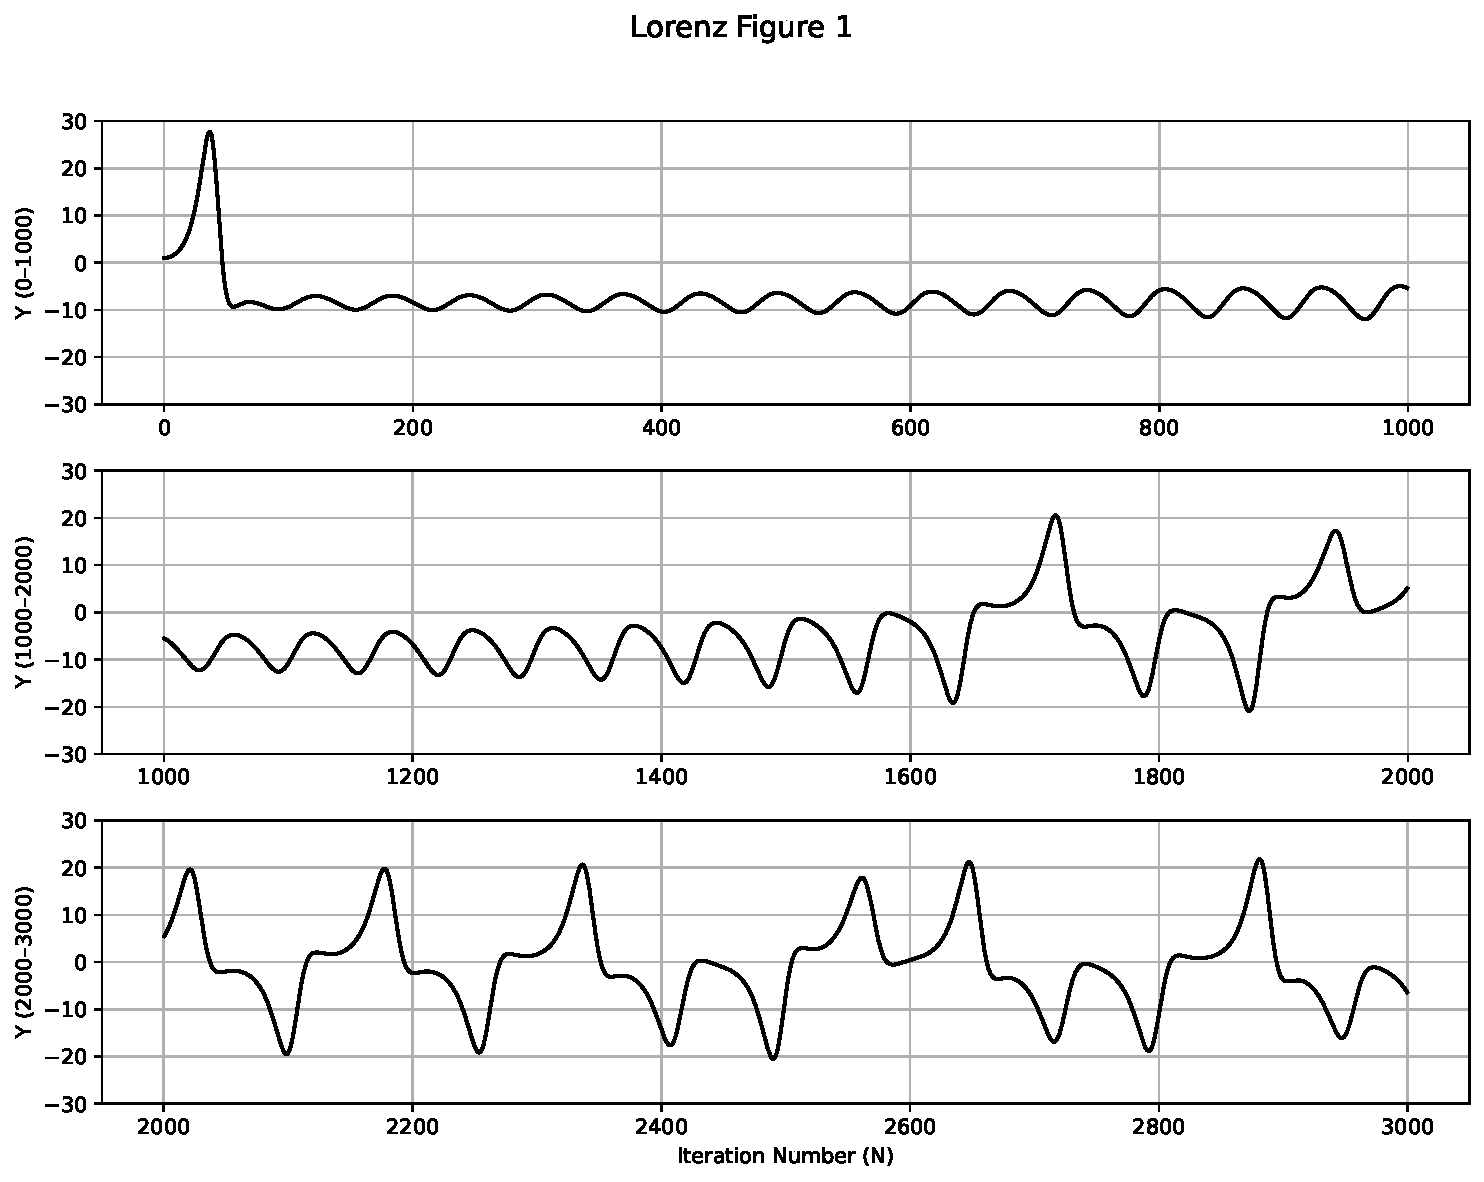
\includegraphics[width=0.85\textwidth]{fig2c.pdf}
    \caption{Reproduction of Lorenz Figure 1: Three successive windows of $Y(t)$, corresponding to iterations 0–3000.}
\end{figure}

\section*{Question 2.4}

To reproduce Lorenz’s Figure 2, we plotted the trajectory in phase space between $t = 14$ and $t = 19$ using a high-resolution sampling of 10,000 time steps. Two projections were shown: $Y$ vs. $Z$ and $Y$ vs. $X$. To match Lorenz’s orientation, the Y-axis in the $Y$–$X$ plot was inverted.

These plots illustrate how the system evolves between different convection states, spiraling around one attractor before transitioning to the other. The looped structure and asymmetry are visual signatures of deterministic chaos in a bounded system.


\begin{figure}[H]
    \centering
    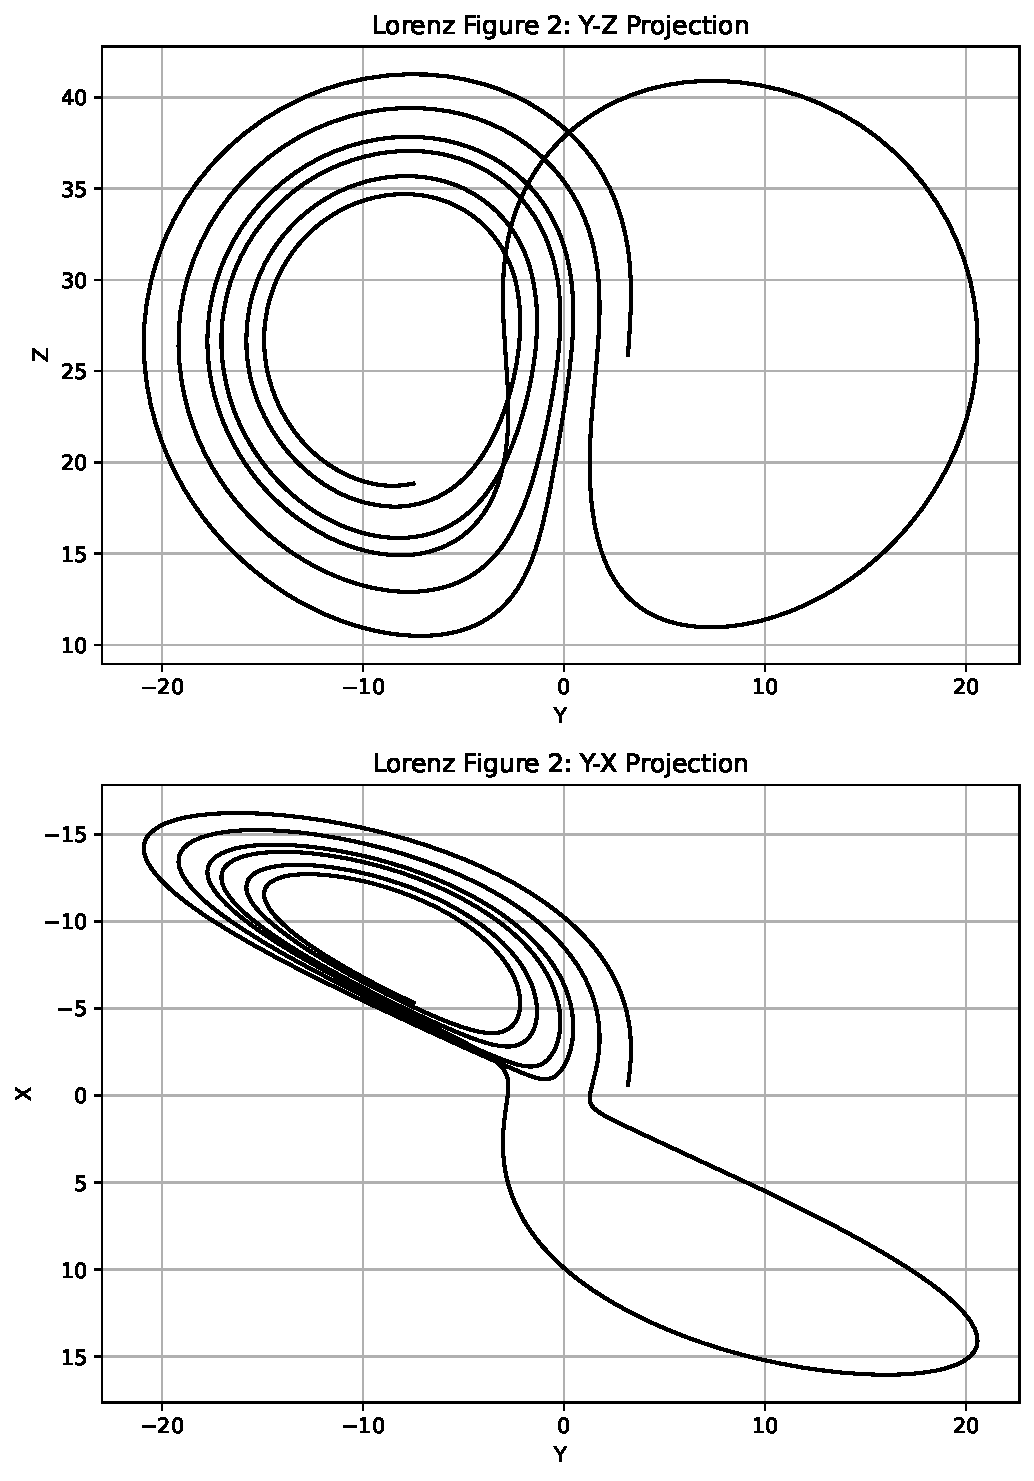
\includegraphics[width=0.8\textwidth]{fig2d.pdf}
    \caption{Reproduction of Lorenz Figure 2: Phase-space projections in the $Y$–$Z$ and $Y$–$X$ planes.}
\end{figure}
\newpage

\section*{Question 2.5: Exponential Divergence}

To demonstrate the sensitivity of the Lorenz system to initial conditions, we repeated the integration using a slightly perturbed initial state: $W_0' = [0., 1.00000001, 0.]$. The system was evolved under the same parameters and over the same time interval as before. This experiment tests the fundamental property of chaos: that nearby trajectories diverge exponentially over time.

We calculated the Euclidean distance between the two solutions, $\| W(t) - W'(t) \|$, at each time step. The resulting distance was plotted on a semilog scale to better visualize the exponential divergence. The semilog plot revealed a clear linear region, consistent with exponential growth of error. After a certain point, the divergence saturates.

In addition, we plotted the raw $Y(t)$ trajectories for both the original and perturbed initial conditions. These appear identical at initial times but diverge visibly after roughly $t = 20$, reinforcing the idea that even minor changes in the initial state lead to drastically different long-term outcomes.

\begin{figure}[H]
    \centering
    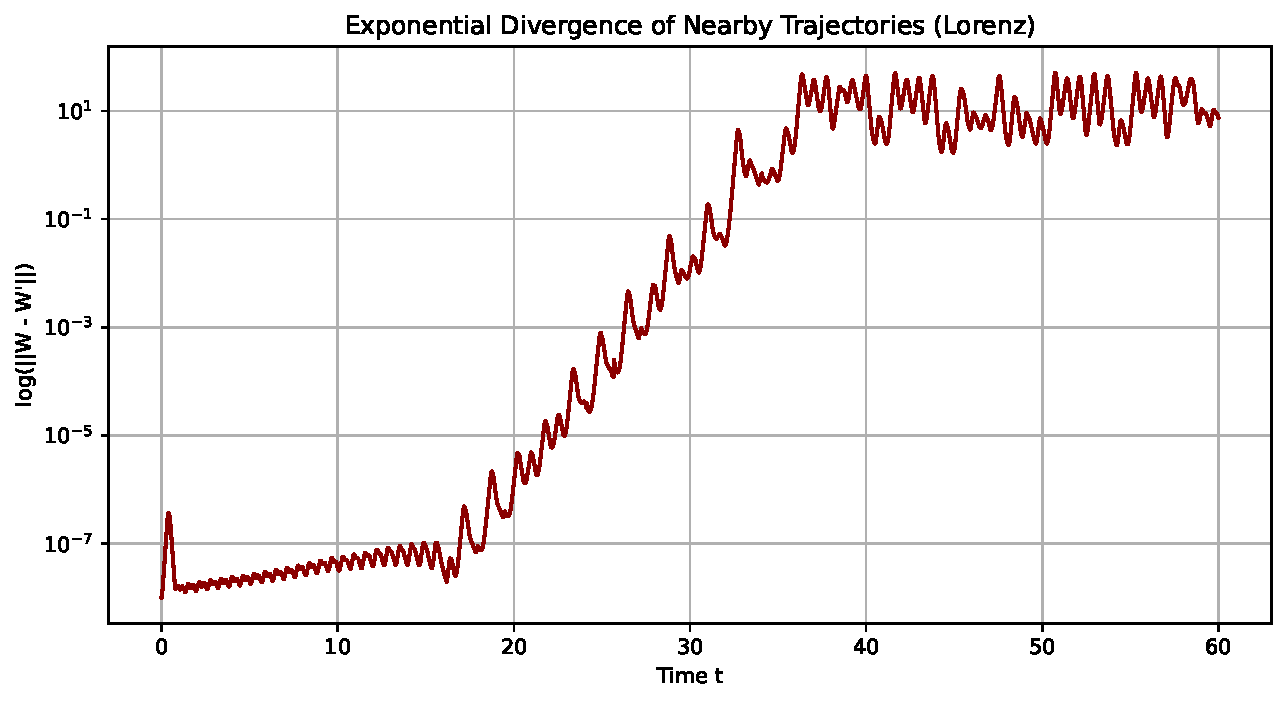
\includegraphics[width=0.85\textwidth]{fig2e.pdf}
    \caption{Exponential Divergence of Nearby Trajectories }
\end{figure}

\end{document}

